\section{FPGA cards as nodes}\label{sec:nodes}

The system is one host with four Alveo U55C cards~\cite{amd_ds978} on PCIe, the same platform as our distributed
statevector simulator~\cite{ali2026multifpga}. As there, each card is a node: it runs its own copy of the kernel, owns
its share of the work, and communicates only with the host. Figure~\ref{fig:nodes} shows the arrangement. What
differs is the work itself. In the statevector simulator a gate on a qubit that indexes the cards needs amplitudes of
other nodes, and the exchange through host memory sets the scaling. In Pauli frame sampling the shots are
independent, so a node needs nothing from any other node. The host's role shrinks to three tasks: compile the circuit
once, load the same program onto every node, and collect the detector and observable bits that the nodes return.

\begin{figure}[t]
\centering
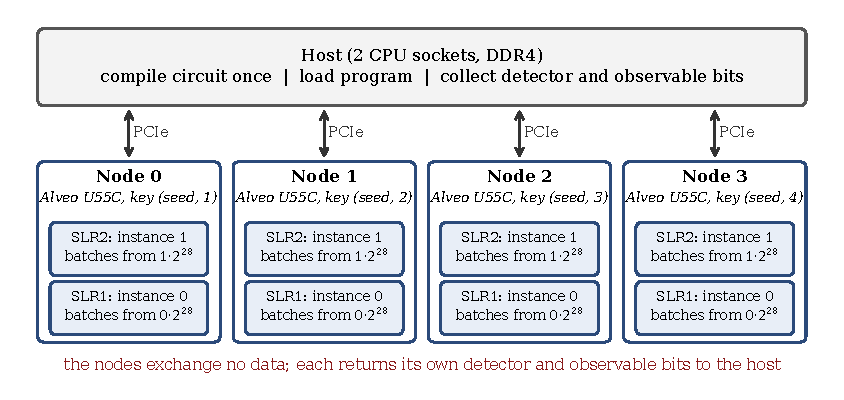
\includegraphics[width=\textwidth]{figures/fig_nodes.pdf}
\caption{Four Alveo U55C cards as nodes of one host. Every card holds \NumInstancesPerCard{} kernel instances, in super
logic regions (SLRs) 1 and 2, each with its own HBM pseudo channels. The host compiles the circuit once, loads the same
program into every instance and receives each instance's detector and observable bits; no data moves between
cards.}\label{fig:nodes}
\end{figure}

\paragraph{Independent random streams.} Independence of the shots only holds if the random numbers of different
nodes are independent. Every noise decision of the kernel is drawn from Threefry4x32-20~\cite{salmon2011random123}, a
counter based generator: its output is a fixed function of a 128 bit counter and a 128 bit key, so any number of
streams can be produced in parallel without shared state, and any single draw can be recomputed in software. Node $c$
uses the key $(s, c+1, 0, 0)$ for a run seed $s$; kernel instance $j$ of a node samples batches $j\cdot 2^{28}$ onwards; and
batch $g$ enters the counter. Two draws of the whole system therefore share a counter and key only if they belong to
the same node, instance, batch, instruction and lane, that is, if they are the same draw. The streams are also
reproducible: the software model of Section~\ref{sec:verification} recomputes the output of any node, instance and
batch from the seed alone, which is how every card is checked bit for bit.

\paragraph{Host side.} One host process per node loads the bitstream, copies the program into every instance once
and then keeps two launches per instance in flight: while one launch runs on the card, the output of the previous
one is copied to host memory. A launch samples a fixed number of batches of \NumLanes{} shots. For measurement, the
processes of all nodes first load their cards and then wait at a common start barrier, so the timed interval of the
system covers the same wall clock window for every node.
